\documentclass[12pt]{article}

\usepackage[utf8]{inputenc}
\usepackage{t1enc}
\usepackage[hungarian]{babel}
\usepackage{graphicx}
\usepackage{geometry}
\usepackage{fancyhdr}
\usepackage{hyperref}
\usepackage{lipsum}
\usepackage{pdfpages}
\usepackage{todonotes}
\usepackage{listings}
\usepackage{xcolor}

\definecolor{codegray}{rgb}{0.5,0.5,0.5}
\definecolor{backcolour}{rgb}{1,1,1}

\lstdefinestyle{codestyle}{
    backgroundcolor=\color{backcolour},   
    numberstyle=\tiny\color{codegray},
    basicstyle=\ttfamily\footnotesize,
    breakatwhitespace=false,         
    breaklines=true,                 
    captionpos=b,                    
    keepspaces=true,                 
    numbers=left,                    
    numbersep=5pt,                  
    showspaces=false,                
    showstringspaces=false,
    showtabs=false,                  
    tabsize=2
}

\lstset{style=codestyle}

\newgeometry{
  top=2.5cm,
  bottom=2.5cm,
  outer=2.5cm,
  inner=2.5cm
}
\linespread{1.25}
\pagestyle{fancy}
\headheight=14.5pt
\fancyhead{}
\lhead{Archytex}
\fancyfoot[C]{\thepage}
\hypersetup{
    colorlinks,
    citecolor=black,
    filecolor=black,
    linkcolor=black,
    urlcolor=black
}


\begin{document}

\begin{titlepage}
  \centering
  
\includegraphics[width=0.15\textwidth]{images/jedlik_logo.png}\par\vspace{1cm}
  {\Large Győri Szakképzési Centrum Jedlik Ányos Gépipari és Informatikai Technikum és Kollégium\par}
  \vspace{2cm}
  
\includegraphics[width=0.25\textwidth]{images/archytex_logo.png}\par\vspace{1cm}
  {\huge\sffamily\textbf{ARCHYTEX}\par}
  \vspace{1cm}
  {\Large Szakdolgozat dokumentáció\par}
  \vfill
  Készítették:\par
  Gulyás Arnold, Marton Zoltán, Szabó Dániel

  \vfill

  \vfill
  % Bottom of the page
  {\large \today\par}
\end{titlepage}

\thispagestyle{empty}

\includepdf[pages=-,pagecommand={},width=\textwidth]{mandatory.pdf}


\tableofcontents

% Introduction
\part{Bevezetés}

Az Archytex egy 3D-s építészeti tervező és látványterv készítő alkalmazás.

Fő célja, hogy egy olyan felületet biztosítson mind professzionális és hobbi szintű felhasználóknak, amely egy építési projekt tervezési folyamatának kezdetétől fogva egészen a látványterv bemutatásáig használható.

Jelentős hangsúly került az optimalizációra, mivel elsődleges szempont volt, hogy gyengébb rendszereken is zökkenőmentesen használható legyen az alkalmazás. Ennek eredményeként született meg a böngészőben futó 3D szerkesztő és a szerveroldali elosztott rendszerű raytracelő renderelőmotor. Így a felhasználó számítógépének erőforrásainak teljes felemésztése nélkül is lehetővé válik az élethű látványtervek készítése.

A letisztult felhasználói kezelőfelület is a könnyű használhatóságot segíti. Regisztráció után bárki hozhat létre projektet, amelyben a beépített eszközök segítségével tervezhet, majd a textúrákat és díszítőelemeket felhasználva életre kelheti építészeti ötleteit. Az alkalmazás könnyedén testreszabható: egy gombnyomással váltható a sötét és világos mód, és a felület több nyelven is elérhető.

Számos olyan alkalmazás létezik, amely építészeti tervezésre vagy látványtervek készítésére szakosodik, de az Archytex-el szemben egyik sem biztosítja az összes funkcionalitást a tervezéstől egészen a látványterv elkészítéséig egy csomagban. Az Archytex használatához nem szükséges semmit letölteni, az összes modern böngészőben futtatható, mivel az egész alkalmazás webes technológiákra épül.

A fejlesztési folyamat során motivációt vettünk több, már létező programból, mint például a Valve Hammer Editor\footnote{\url{https://developer.valvesoftware.com/wiki/Valve\_Hammer\_Editor}} (objektumok és textúrák megjelenítése), a Blender\footnote{\url{https://www.blender.org/}} (objektum transzformációk billentyűkombinációi) vagy az Unreal Engine\footnote{\url{https://www.unrealengine.com/}} (navigáció a szerkesztő 3D terében). Ezen programok funkciója és célközönsége nagyban különbözik az Archytex-étől, viszont egyes elemeket és ötleteket átemelve kiválóan kiegészítik alkalmazásunk funkcionalitását.

Az Archytex elérhetőségei:
\begin{itemize}
  \item Weboldal: \url{https://archytex.tech}
  \item GitHub repository: \url{https://github.com/Texyfore/Archytex}
\end{itemize}

\part{Felhasználói dokumentáció}
\rhead{}

% Account
\section{Felhasználói fiók}
\rhead{Felhasználói fiók}

\subsection{Regisztráció}
Az Archytex alkalmazásban a szolgáltatások használatához felhasználói fiók létrehozására van szükség. Ez a honlapon a \emph{/register} útvonalon vagy a bejelentkezés oldalon a \emph{Csatlakozz az Archytex-hez} link használatával elérhető regisztrációs lapon tehető meg.

\begin{samepage}
  \noindent Regisztrációhoz szükséges adatok:
  \begin{itemize}
    \item Felhasználónév
    \item E-mail cím
    \item Jelszó
  \end{itemize}
\end{samepage}

\begin{figure}[h]
  \centering
  
\includegraphics[scale=.5]{parts/user-documentation/account/images/register.png}
  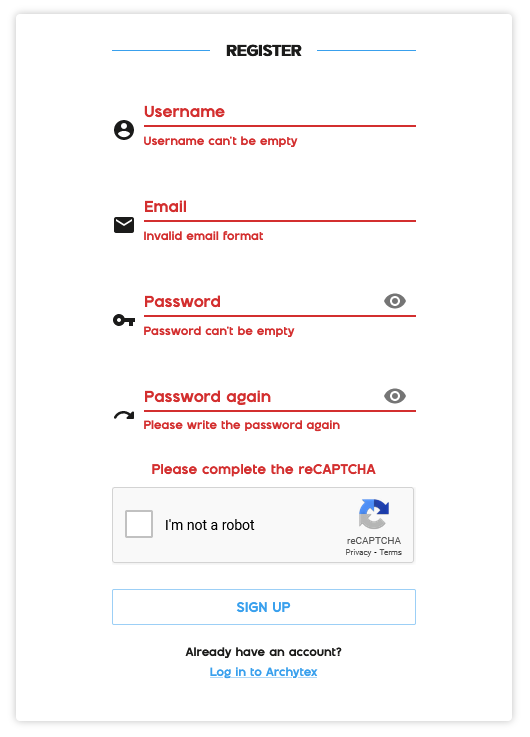
\includegraphics[scale=.5]{parts/user-documentation/account/images/register-errors.png}
  \caption{A regisztrációs űrlap és a hibaüzenetek kijelzése}
\end{figure}

A regisztrációs és a bejelentkezési űrlapon is történik hibakezelés, így nem adható meg hibás adat. Új fiók létrehozása után a megadott e-mail címre küldött levélben található linkkel erősíthető meg a regisztráció.

\subsection{Bejelentkezés}
A bejelentkezési képernyő a honlapon a \emph{/login} útvonalon vagy asztali nézeten a navigációs csík jobb oldalán található \emph{Bejelentkezés} gombbal, telefonos nézeten pedig a hamburger ikonnal kinyitható navigációs menüben található \emph{Bejelentkezés} gombbal érhető el. Bejelentkezés csak a már regisztrált és a regisztrációt megerősített fiókokkal lehetséges.

\begin{figure}[h]
  \centering
  
\includegraphics[scale=.6]{parts/user-documentation/account/images/login.png}
  
\includegraphics[scale=.6]{parts/user-documentation/account/images/login-errors.png}
  \caption{A bejelentkezési űrlap és a hibaüzenetek kijelzése}
\end{figure}

\subsection{Felhasználók számára elérhető funkciók}
Bejelentkezés után a felhasználó számára elérhetővé válnak az Archytex által nyújtott szolgáltatások. Megjelenik a navigációs csíkon a vezérlőpult; itt lehetséges új projektek létrehozása, valamint a projektek megnyitása a szerkesztőben. Úgyanúgy a navigációs csíkon található a jobb oldalon a profil ikon, amelyre kattintva egy menü nyitható meg. Ezen menüben található a \emph{Beállítások} és a \emph{Kijelentkezés} gomb.

A szekesztőben készített jelenetek elmenthetőek a fejlécben található \emph{Mentés} gombbal. A projekt következő megnyitásakor az elmentett állapot fog megjelenni. Emellett lehetőség van az elkészített jelenetek renderelésére. Egy projekthez tartozó renderek a vezérlőpulton a projekt lenyitása után tekinthetőek meg.

% Dashboard
\section{Vezérlőpult}
\rhead{Vezérlőpult}

% Editor
\section{Szerkesztő}
\rhead{Szerkesztő}

\subsection{Technológiák}

A 3D szerkesztő elkészítése számos technikai és tervezési problémát vetett fel. Egy olyan szoftver
megalkotása volt a cél, amely elég egyszerű ahhoz, hogy bárki használhassa, viszont megfelelően
eszköz dús ahhoz, hogy képes legyen bonyolult épületek tervezésére is. Ezen feltételek
megfogalmazása után arra jutottunk, hogy a 3D szerkesztőt egy web alapú alkalmazás keretein belül
fogjuk megvalósítani.

Egy ilyen szoftver esetében nagyon fontos a sebesség, ezért úgy döntöttünk, hogy a
böngészőkben használt JavaScript helyett a sokkal gyorsabb --- ámbár fiatalabb és éretlenebb ---
WebAssembly\footnote{\url{https://webassembly.org}} technológiát fogjuk használni. Mivel a
WebAssembly önmagában csak egy utasításkészlet, szükségünk volt egy programozási nyelvre,
amit lehetséges WebAssembly utasításokra fordítani. Erre a célra a
Rust\footnote{\url{https://www.rust-lang.org}}
programozási nyelvet választottuk. Ennek a döntésnek több oka is van:

\begin{itemize}
      \item Gyorsaság: A Rust egy rendszerközeli nyelv, hasonlóan a C-hez vagy C++-hoz, így rengeteg
            olyan optimalizáció valósítható meg, ami magasabb szintű nyelvekben nem lehetséges.

      \item Fejlett WebAssembly eszközök: Annak ellenére, hogy a nyelv viszonylag fiatal, rengeteg
            kiváló eszköz és könyvtár áll rendelkezésre a WebAssembly programok fejlesztésének
            elősegítéséhez. Ezek közül talán a legfontosabb a
            wasm-bindgen\footnote{\url{https://github.com/rustwasm/wasm-bindgen}} könyvtár, amellyel
            triviális feladattá válik a böngésző által használt JavaScript kód és a WebAssemblyre
            átforduló Rust kód összekötése.

      \item Tapasztalat: A fejlesztői csapat két tagja már használta a Rust programozási nyelvet a
            múltban, így elkerülhettük az új technológiák tanulásával járó problémákat.
\end{itemize}

\subsection{Működési elvek}

A használt technológiák kiválasztása után megkezdődött a szerkesztő működési elveinek felállítása.
Hamar eldöntöttük, hogy nagyrészt két, már létező szoftver eszközeiből szeretnénk ötleteket
meríteni.

Az egyik szoftver, a Blender egy általános rendeltetésű
háromdimenziós modellező program. Rendkívül sokoldalú és bonyolult, ezért csak néhány mechanizmust
ültettünk át a saját szerkesztőnkbe, például a kijelölés és a mozgatás módját.

\begin{figure}[H]
      \centering
      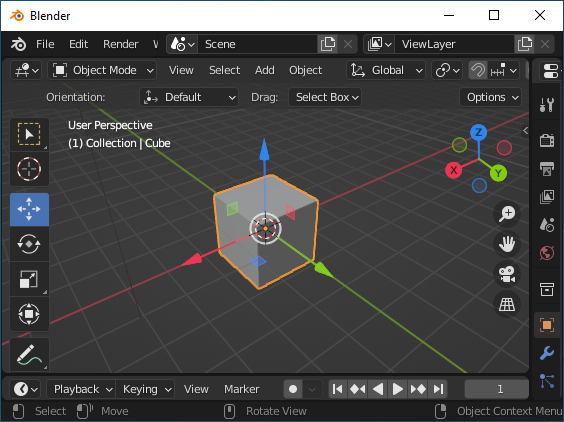
\includegraphics[width=0.5\textwidth]{parts/developer-documentation/editor/images/blender.png}
      \caption{Blender}
\end{figure}

A másik kiindulási pontként használt szoftver a Valve Hammer Editor. A
program a Valve Software által fejlesztett Source játékmotor pályaszerkesztő alkalmazása. A Hammer
Editor egyik erőssége, és egyben az a tulajdonsága, amit mi is megvalósítottunk az, hogy benne
bármilyen komplex beltéri vagy kültéri jelenet lemodellezhető kisebb, egyszerűbb alakzatok
felhasználásával.

\begin{figure}[H]
      \centering
      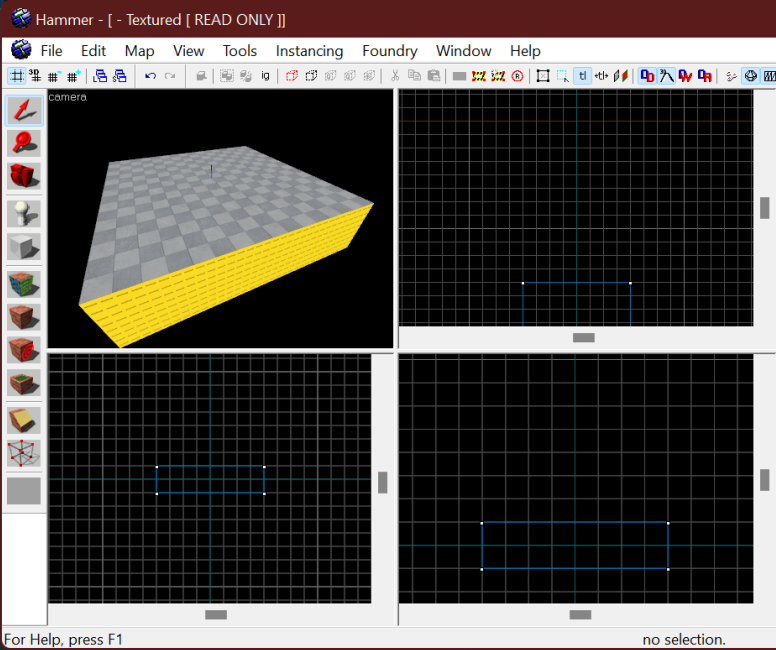
\includegraphics[width=0.5\textwidth]{parts/developer-documentation/editor/images/hammer.png}
      \caption{Valve Hammer Editor}
\end{figure}


\subsection{Kommunikáció a böngészővel}

Problémák és kihívások nem csak a tervezési fázisban bukkantak fel. Az egyik legelső probléma,
amivel fejlesztés közben találkoztunk, az a böngészővel való kommunikáció kérdése. Mivel a
JavaScript alapú felhasználói felület, és a Rust alapú szerkesztő valójában két független
alkalmazás, ezért ki kellett találni egy módszert az információmegosztásra. Az egyszerű
függvényhívások két okból nem feleltek meg. Először is, a JavaScript és WebAssembly kód natívan
csak egész számok átadására képes, ami mi céljainkhoz kevés. Másodszor, mivel a szerkesztő teljes
mértékben WebAssembly memóriában él, nincs semmilyen JavaScript objektum, aminek a függvényeit le
lehetne hívni.

Az első problémánkra a wasm-bindgen nevű Rust könyvtár adott megoldást. A wasm-bindgen lehetségessé
teszi az egész számoknál komplexebb adatstruktúrák átültetését Rust kódból JavaScript kódba, és
fordítva. A második probléma megoldása kicsit nehezebbnek bizonyult. Végül egy olyan
modellt valósítottunk meg, amiben a két fél két különböző módszert használ a kommunikációhoz.
Amikor a böngésző kommunikál a szerkesztővel, azt üzenetekkel teszi. Ezek az üzenetek egyszerű
adatstruktúrák amik egy aszinkron csatornán keresztül jutnak el a szerkesztőhöz. Amikor az
információátadás fordítva történik, a helyzet egyszerűbb: a JavaScript oldal egyszerűen átad egy
anonim függvényt a Rust oldalnak, amit aztán a szerkesztő szükség esetén meghív.

\subsection{3D grafika}

A szerkesztő egyik legfontosabb feladata, hogy képes legyen kirajzolni a jelenetet a képernyőre.
Ezt teszik lehetővé a különböző grafikus API-k, mint például az
OpenGL\footnote{\url{https://www.opengl.org}}, Vulkan\footnote{\url{https://www.vulkan.org}},
vagy böngésző esetén a WebGL\footnote{\url{https://www.khronos.org/webgl}}.
A Rust programozási nyelvhez rengeteg olyan könyvtár érhető el, ami ezeket az API-ikat elérhetővé
teszi. Mi úgy döntöttünk, hogy a wgpu\footnote{\url{https://github.com/gfx-rs/wgpu}} könyvtárat fogjuk
használni. Ennek legfőbb oka az, hogy egy letisztult, biztonságos réteget húz a régies WebGL
interfészre.

\pagebreak

\subsection{Művelet alapú szerkesztés}

Az előzetes tervezési fázisban számunkra fontos kikötés volt, hogy a szerkesztés közben
megvalósulhasson az ún. non-destruktív munkamenet. Ez azt jelenti, hogy bármit, amit a felhasználó
megtesz, azt vissza lehet vonni. Ahhoz, hogy ez lehetséges legyen, valamilyen formában el kell
tárolni a múltbeli szerkesztési lépéseket. Végül úgy döntöttünk, hogy az egész szerkesztőt ezen
alapelv köré építjük fel. Létrehoztunk egy speciális adatszerkezetet, amely az összes elvégezhető
szerkesztési lépést képes eltárolni. Amikor a felhasználó változtat valamit a jeleneten, egy
ilyen adatszerkezet (művelet) kerül átadásra. Az végrehajtás után a szerkesztő felépíti az művelet
ellentétét, az inverz műveletet. Végül az inverz művelet eltárolásra kerül egy ún. visszavonási
veremben. Amikor a felhasználó kiadja a visszavonási parancsot, a visszavonási verem tetején lévő
művelet (ha létezik) újra végrehajtásra kerül, és belekerül egy másodlagos verembe, ami a visszavont
műveletek inverzeit tárolja. Ez azért szükséges, mert visszavonás mellet ismétlés is lehetséges.

\begin{figure}[H]
      \centering
      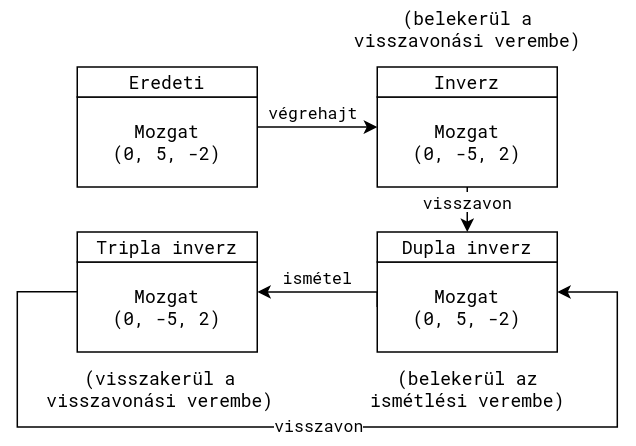
\includegraphics[width=0.5\textwidth]{parts/developer-documentation/editor/images/actions.png}
      \caption{A művelet alapú szerkesztés folyamatábrája}
\end{figure}

\subsection{Külső erőforrások kezelése}

A tervezési fázisban hamar kiderült, hogy sok időt és energiát kell fektetnünk a szerkesztő által
használt külső erőforrások tárolásának és létrehozásának módjának meghatározásába. Arra jutottunk,
hogy ezen célok teljesítéséhez saját fájlformátumokat fogunk kifejleszteni. A fejlesztés során
felmerülő igények kielégítésére végül három új fájlformátum született meg: .ascn, .amdl, és .agzm.
Mindhárom fájlformátum bináris kódolású, előállításukat és beolvasásukat a
bincode\footnote{\url{https://github.com/bincode-org/bincode}}
könyvtár végzi. Az adatokat mindegyik formátum egymásba ágyazott struktúrákban tárolja.

\pagebreak

\subsubsection{Jelenetfájl (.ascn)}

Az első általunk fejlesztett fájlformátum, a .ascn arra szolgál, hogy a szerkesztőben készített
3D jeleneteket tárolja. Az egész adatszerkezet egyetlen \emph{Scene} nevű struktúrában helyezkedik
el. Ennek a struktúrának két eleme van: \emph{camera} és \emph{world}. A \emph{Camera} struktúrában
a kamera pozíciója és forgása tárolódik, míg a \emph{World} struktúra kicsit bonyolultabb. Szintén
két eleme van: \emph{solids} és \emph{props}. Mindkét elem vektoros adatszerkezet, azaz
határozatlan mennyiségű homogén adatot tárol.

A \emph{solids} elem \emph{Solid} típusú struktúrákat tárol. Egy \emph{Solid} példány egy primitív
szilárd alakzatot modellez. Tartalmazza az alakzat csúcsait és lapjait, emellett a lapok textúráit.

A \emph{props} elem \emph{Prop} típusú struktúrákat tárol. Egy \emph{Prop} példány egy díszítőelem
adatait tárolja. Egy díszítőelemnek modell ID-je, pozíciója és forgása van.

\begin{figure}[H]
      \centering
      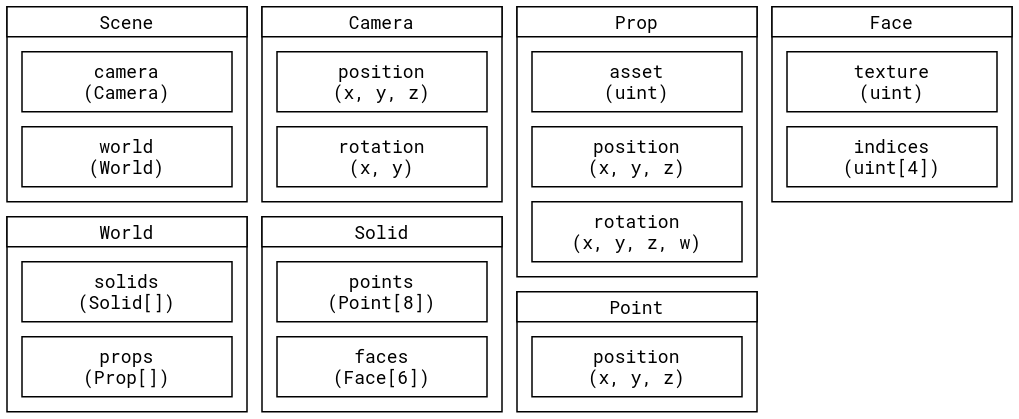
\includegraphics[width=0.8\textwidth]{parts/developer-documentation/editor/images/ascn.png}
      \caption{A .ascn fájlformátum adatszerkezetei}
\end{figure}

\pagebreak

\subsubsection{Modellfájl (.amdl)}

A .amdl fájlformátum egy tetszőlegesen komplex 3D modell tárolására szolgál, néhány korlátozással.
A formátum például nem képes animációkat kódolni, hiszen a szerkesztő nem támogatja a mozgó tárgyak
megjelenítését. A modellfájl gyökérstruktúrája \emph{Prop} névre hallgat. Két eleme van:
\emph{bounds} és \emph{meshes}. A \emph{bounds} elem a modell köré írható,
tengelyekhez igazított téglatestet tárolja. A \emph{meshes} elem vektoros adatszerkezet, ami a
modellt felépítő, textúrázott almodelleket tárolja.

\begin{figure}[H]
      \centering
      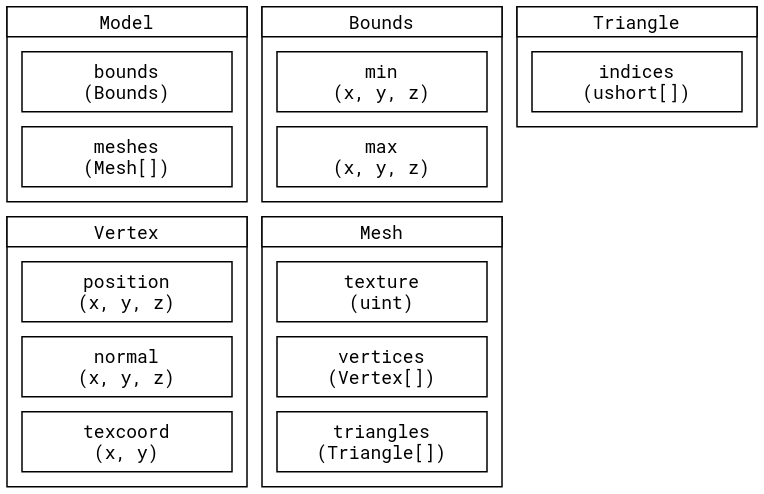
\includegraphics[width=0.6\textwidth]{parts/developer-documentation/editor/images/amdl.png}
      \caption{A .amdl fájlformátum adatszerkezetei}
\end{figure}

\subsubsection{Gizmofájl (.agzm)}

Az Archytex szerkesztő forráskódjában a gizmo szónak két jelentése is van: hivatkozhat az egér
általi mozgatást elősegítő alakzatokra, de arra a speciális 3D modellre is, aminek nincsenek
almodelljei és textúrái sem. A gizmofájl az utóbbi modellek tárolására szolgál. A három saját
fájlformátum közül ez a legegyszerűbb, hisz csak egyszerű geometriát kódol: csúcsokat, és az
azokból alkotott háromszögeket.

\begin{figure}[H]
      \centering
      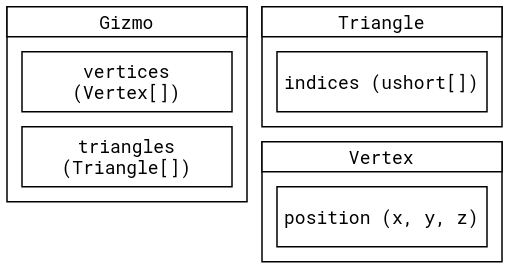
\includegraphics[width=0.4\textwidth]{parts/developer-documentation/editor/images/agzm.png}
      \caption{A .agzm fájlformátum adatszerkezetei}
\end{figure}

\part{Fejlesztői dokumentáció}
\rhead{}

% Work
\section{Munkamegosztás}
\rhead{Munkamegosztás}

\subsection{Feladatok elosztása}
Az Archytex projektet három fős csapatban készítettük, ezért fontos volt számunkra, hogy az elejétől fogva tiszta legyen, hogy kinek mi a feladata. Mindegyikünk különböző technológiákban jártas, és máshoz ért, így egymás tudását kiegészítve egy összetett applikációt tudtunk készíteni. Gulyás Arnold a 3D grafikához ért a legjobban, ezért ő felelt a szerkesztőért. Marton Zoltán feladata volt a backend fejlesztése, az adatbázis felépítése és a ray-tracer elkészítése. Szabó Dániel feladata volt az alkalmazás design tervének elkészítése és a frontend programozás.

\subsection{Verziókezelés}
A projekt folyamán gyakran párhuzamosan dolgoztunk, és szerettük volna figyelemmel követni, hogy hogyan épül fel az alkalmazás, ezért a GitHub nevű git verziókezelő szolgáltatást használtuk.

Szabályosan követtük a vállalatoknál is jellemző git használati kultúrát: issue-kat készítettünk és minden issue-t külön ágon programoztunk le, ami után a fő ágba, a master-be \emph{pull request} használatával beolvasztottuk az issue ágát.

\begin{figure}[h]
  \centering
  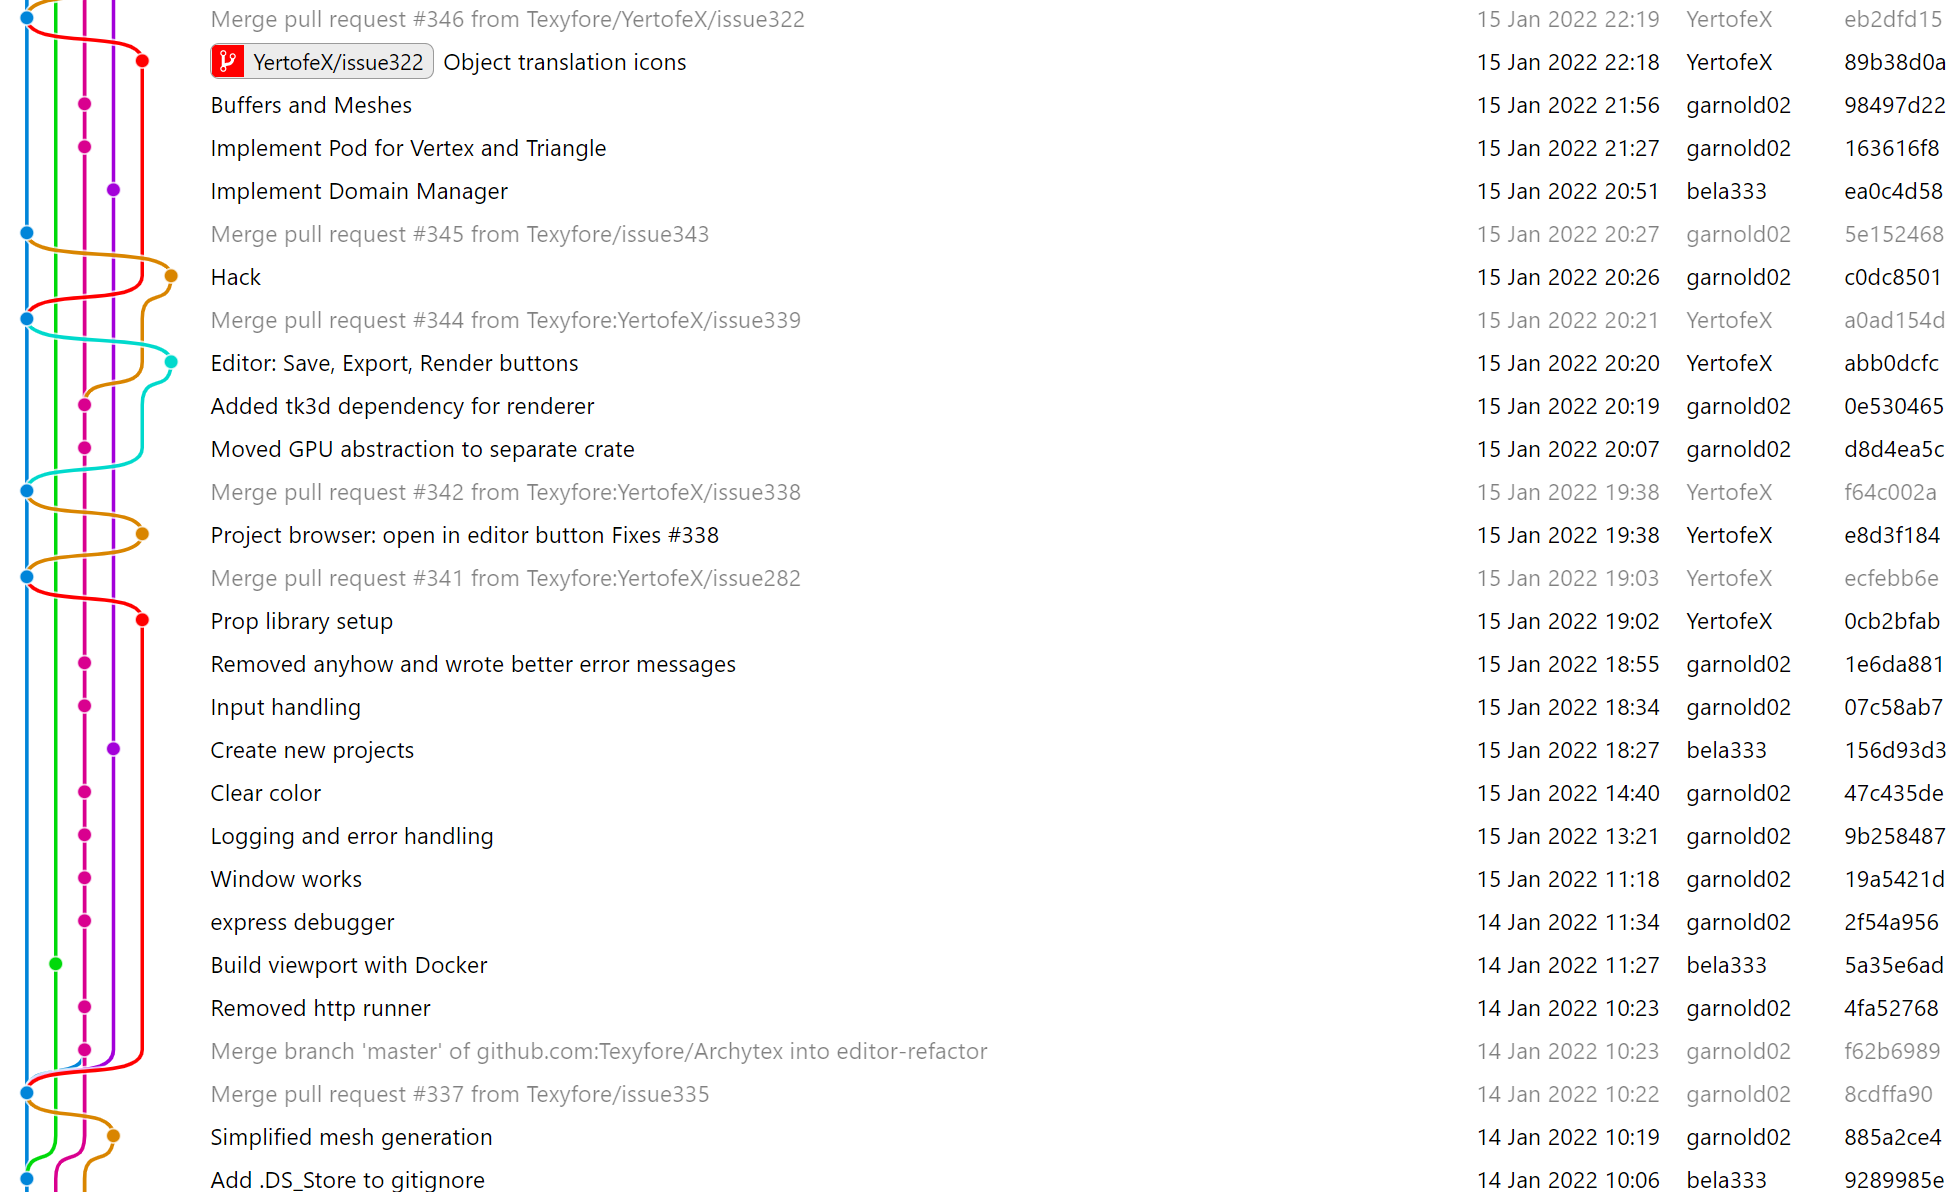
\includegraphics[width=.9\textwidth]{parts/developer-documentation/work/images/git-history.png}
  \caption{Git history képernyőkép}
\end{figure}

\subsection{GitHub használata}
Az Archytex projektet egy GitHub repository-ban fejlesztettük. Ez lehetővé tette, hogy bárhonnan, bármilyen gépről tudjuk fejleszteni az applikációt.

\begin{figure}[h]
  \centering
  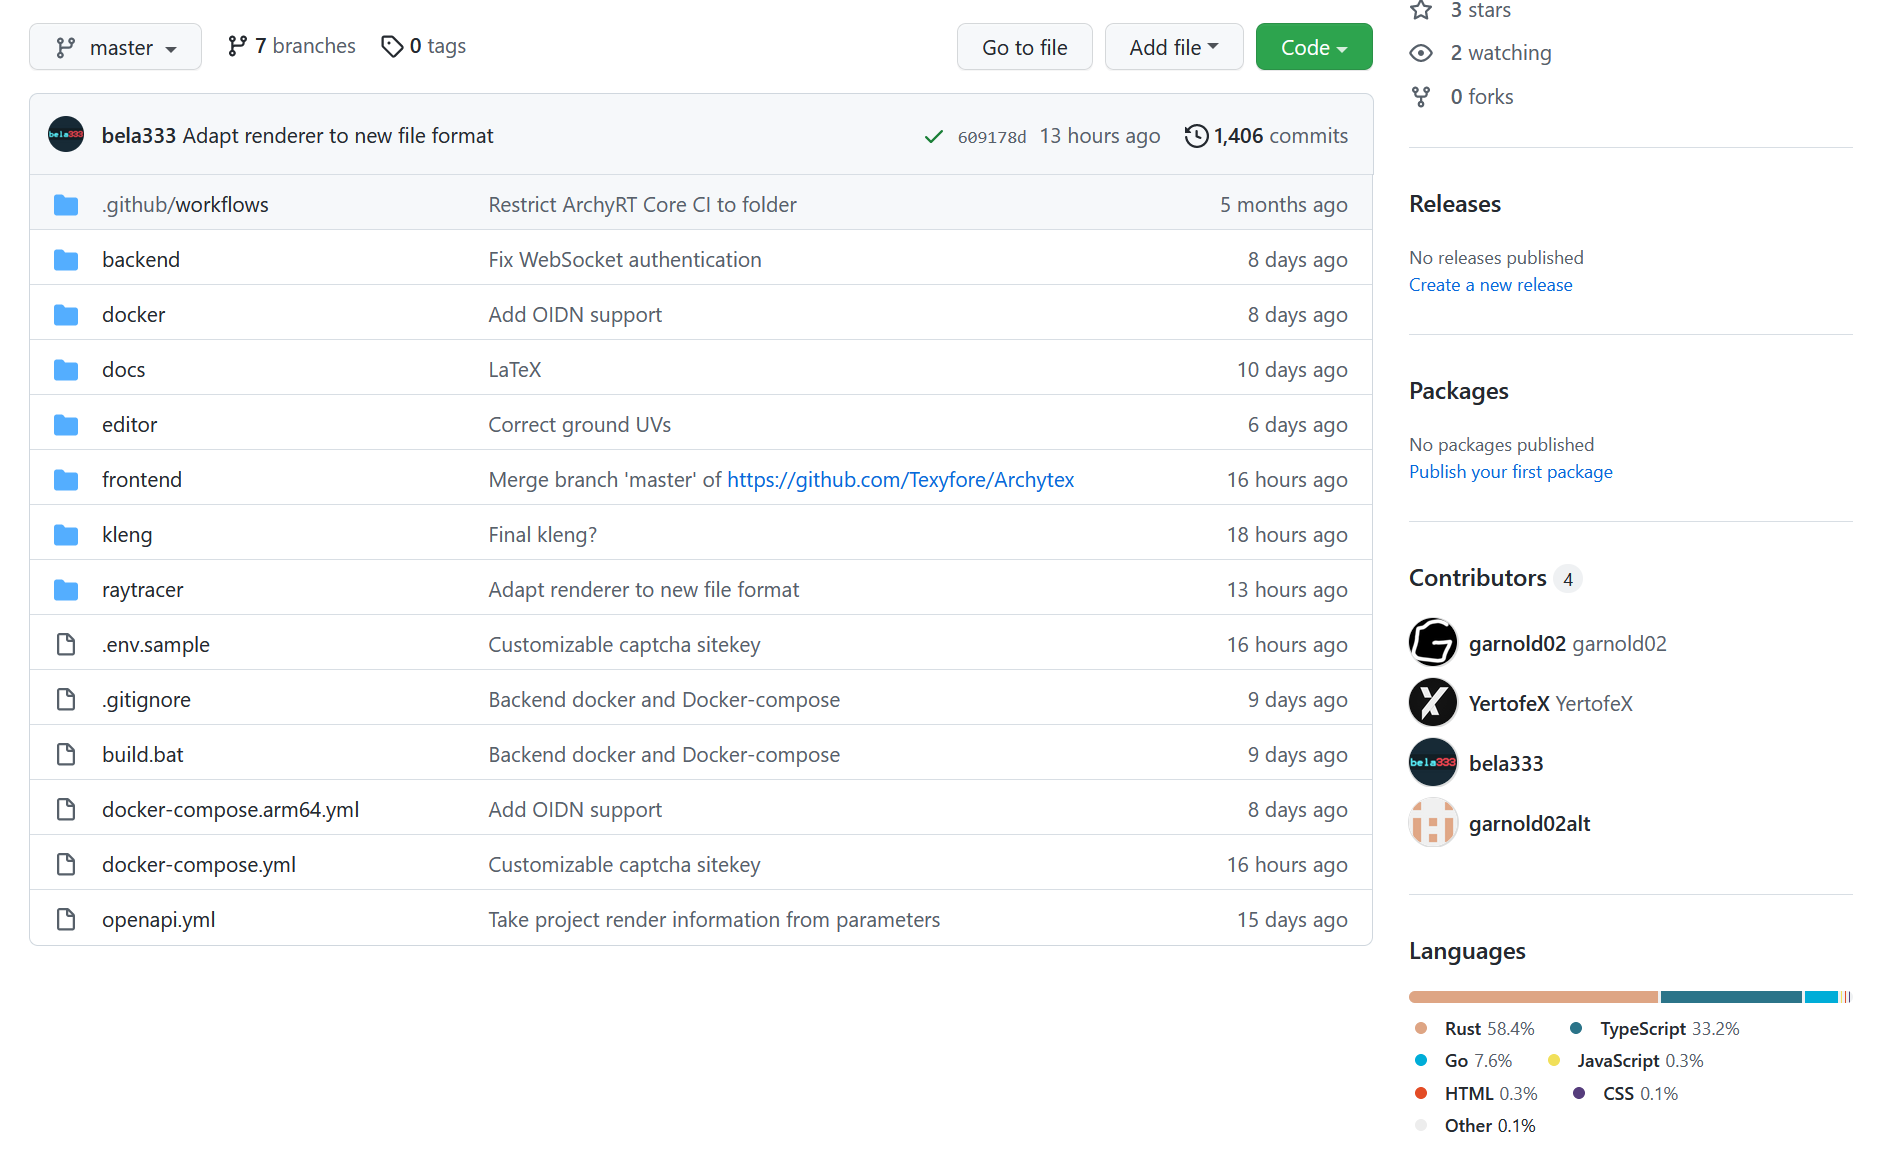
\includegraphics[width=.9\textwidth]{parts/developer-documentation/work/images/repository.png}
  \caption{Az Archytex repository képernyőképe}
\end{figure}

Hogy követni tudjuk, kinek milyen feladata van, létrehoztunk egy kanban\footnote{Kanban: 'elkészítendő', 'folyamatban' és 'elkészült' oszlopokból álló, 3 oszlopos feladattábla} típusú táblát GitHub-on, ahol az issue-kat kártyák formájában tudtuk kezelni. A kártyák kategorizálására címkéket használtunk, az ütemterv betartásának segítéséhez pedig mérföldköveket.

\begin{figure}[h]
  \centering
  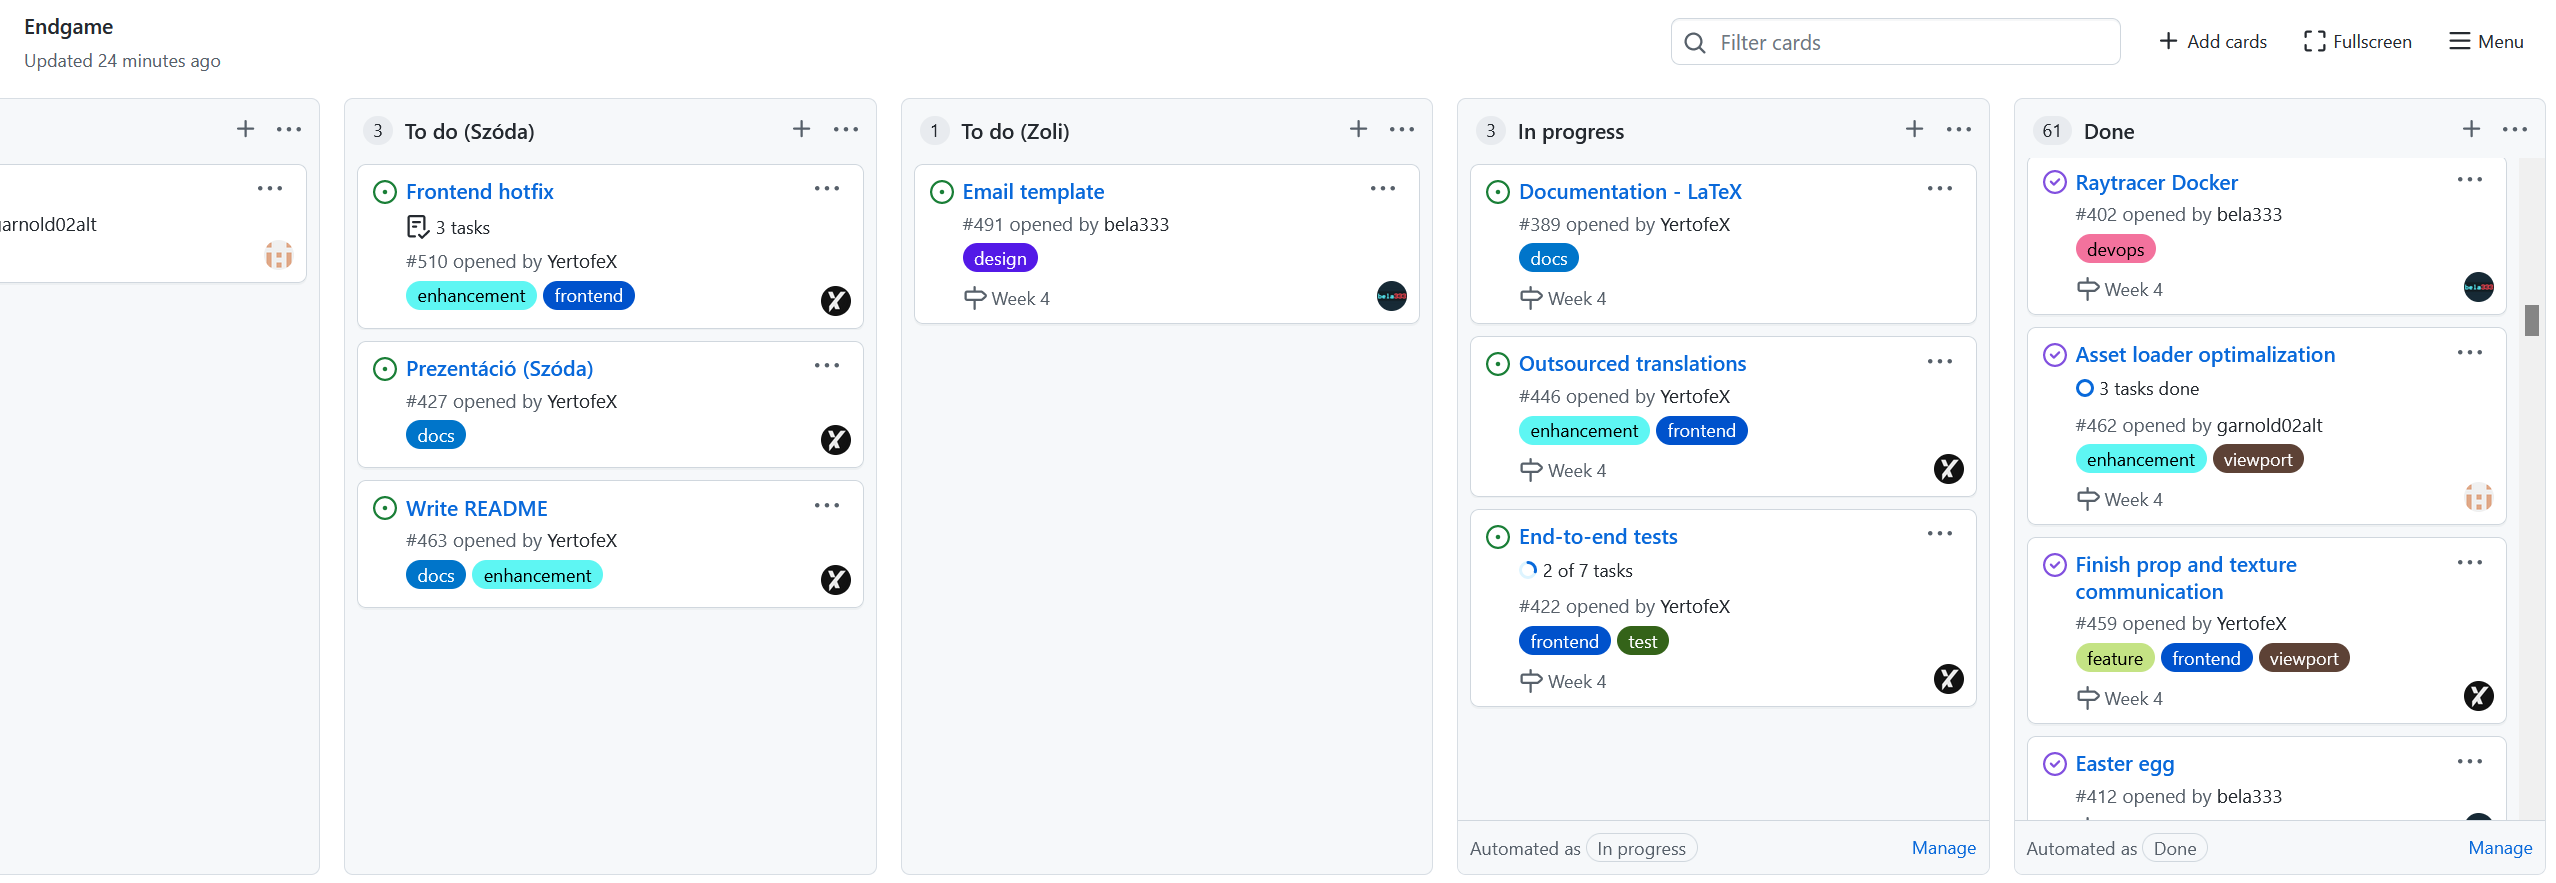
\includegraphics[width=.9\textwidth]{parts/developer-documentation/work/images/github-project.png}
  \caption{Projekt nézet az Archytex repository-ban}
\end{figure}

\subsection{Statisztikák}

\begin{figure}[h]
  \begin{center}
    \begin{tabular}{|c|c|c|}
      \hline
      Commit-ok & Issue-k & Pull request-ek \\
      \hline
      1406      & 293     & 217             \\
      \hline
    \end{tabular}
    \caption{Az Archytex projekt számokban}
  \end{center}
\end{figure}

\begin{figure}[h]
  \centering
  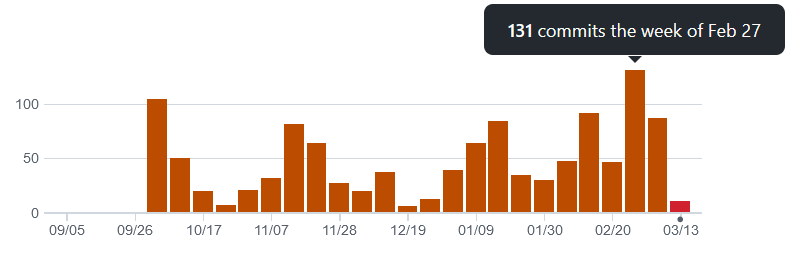
\includegraphics[width=.82\textwidth]{parts/developer-documentation/work/images/commits.png}
  \caption{Commit-ok heti felbontásban 2021. szeptemberétől 2022. márciusáig}
\end{figure}

\begin{figure}[h]
  \centering
  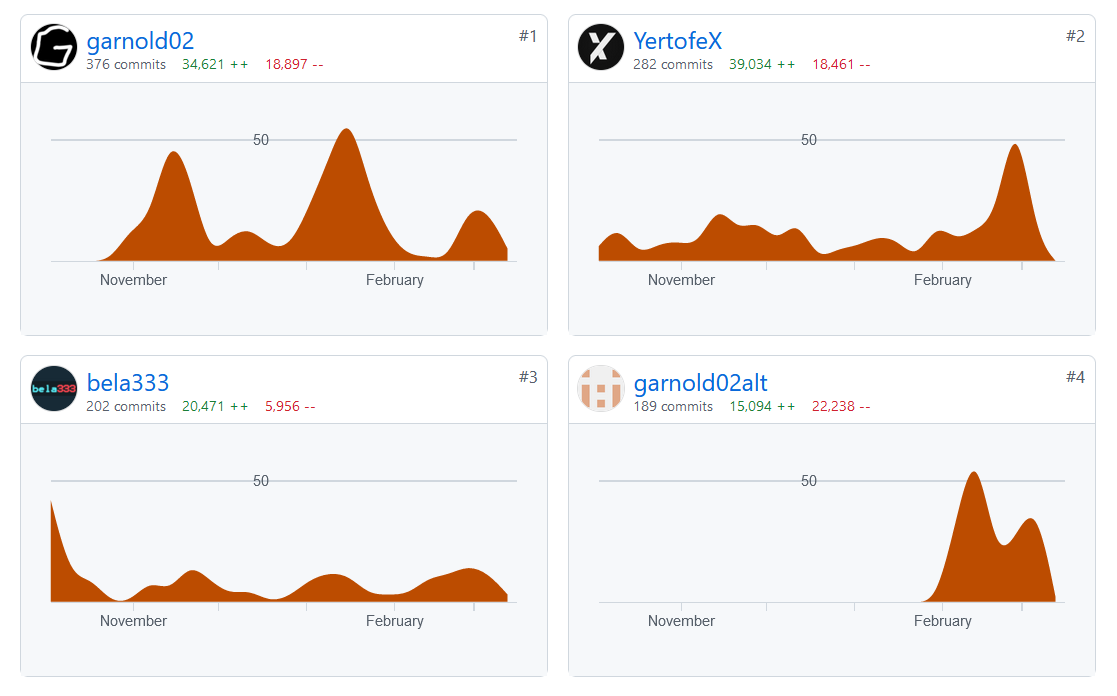
\includegraphics[width=.65\textwidth]{parts/developer-documentation/work/images/commit-frequency.png}
  \caption{Commit-ok eloszlása a csapattagok között.}
\end{figure}

% Backend
\section{Backend}
\rhead{Backend}
\subsection{Használt technológiák}
A backend megírásánál az egyszerűségre és a későbbi könnyebb felhasználhatóságra törekedtünk, így esett választásunk a Go-MongoDB stack-re.
\subsubsection{MongoDB}
A \emph{MongoDB}\footnote{\url{https://www.mongodb.com/}} egy NoSQL adatbázis, amely annyit tesz, hogy táblák és sorok helyett egy JSON szerű struktúrában tárolja el az adatokat.
Ennek több előnye és hátránya is van.

\begin{samepage}
\noindent Előnyei:
\begin{itemize}
    \item Egyszerű feltöltés/letöltés a JSON szerű formátum miatt
    \item Nem szükséges előre felépíteni az adatbázis struktúráját
    \item Frissítések valós-idejű figyelése
\end{itemize}

\noindent Hátrányai:
\begin{itemize}
    \item Ritkábban használt
    \item Átlagoshoz képest komplexebb lekérdezések
    \item Sémának való megfelelés nem ellenőrzött
    \item Kevésbé rendezett, mint a relációs adatbázisok
\end{itemize}
\end{samepage}

Az említett valós-idejű figyelés, amely a projekt frissítéséhez szükséges, csak replica set esetén működik, tehát akkor ha a szerver be van állítva a megosztott munkára.
\subsubsection{Go}
A stack másik tagja, a \emph{Go}\footnote{\url{https://golang.org/}} egy programozás nyelv, amelyet a Google fejlesztett ki. A cél egy átlátható, egyszerű nyelv készítése volt, amelyet a \emph{Python}-t használó fejlesztők is könnyen megtanulhatnak. \todo[inline]{Citation: Tényleg a python developerek miatt készült?}

\begin{samepage}
\noindent Előnyei:
\begin{itemize}
    \item Típusos, így kisebb az esélye a hibáknak
    \item Erős beépített web fejlesztési (HTTP, sablonok stb.) könyvtárak
    \item Egyszerű párhuzamos futtatás \emph{Goroutine}-okkal és csatornákkal
    \item Fordított, de szemétgyűjtős
    
\end{itemize}
\end{samepage}

\begin{samepage}
\noindent Hátrányai:
\begin{itemize}
    \item Adatfeldolgozási függvényekben hiányos
    \item Generikusok hiánya
    \item Frusztrálóan bőszavú hibakezelés
\end{itemize}
\end{samepage}

Az e-mail rendszerhez a beépített net/smtp \todo{Acronym} könyvtárat használtuk az üzenetek elküldéséhez, illetve a html/template könyvtárat az üzenetek tartalmának kitöltéséhez.

A fejlesztésben sokat segített a \emph{Gorilla} könyvtár, amely az alapértelmezett HTTP könyvtárat egészíti ki további hasznos funkcióval.
Például middleware támogatással, metódus korlátozással, URL-be helyezett paraméterekkel stb.

\subsection{Szolgáltatások méretezése}
A \emph{docker-compose} fájlban található \emph{Traefik}\footnote{\url{https://traefik.io/traefik/}} két fő feladatot lát el:

\begin{samepage}
\begin{itemize}
    \item Statikus frontend fájlok és a Backend api egy végpontra helyezése
    \item Automatikus terheléselosztás
\end{itemize}
\end{samepage}

A \emph{Traefik} beintegrálja magát a \emph{Docker}-be és így látja, ha egy szolgáltatásból több fut és el tudja közöttük osztani a terhet.

Ha szeretnénk egy szolgáltatást méretezni, akkor a \emph{docker-compose} parancsot kell lefuttatnunk, a következő parancsok egyikével:

\begin{itemize}
    \item Statikus fájl szerver méretezése
    \begin{lstlisting}[language=bash]
        $ docker-compose up --scale frontend=<DARAB>
    \end{lstlisting}
    \item Backend szerver méretezése
    \begin{lstlisting}[language=bash]
        $ docker-compose up --scale backend=<DARAB>
    \end{lstlisting}
\end{itemize}
    

\todo[inline]{Adatbázis model}
\todo[inline]{HTTP dokumentáció}
\todo[inline]{WS dokumentáció}

% Frontend
\section{Frontend}
\rhead{Frontend}

A frontend a szoftver azon része, amely nagyban meghatározza egy felhasználó élményét. Fontos az átláthatóság, a könnyű kezelhetőség és az esztétika. Ezen szempontokat figyelembe véve készítettük el az Archytex weboldalt.

\subsection{Design terv}
A honlap elkészítésének első lépése a tervezés volt. Ehhez a Figma\footnote{\url{https://www.figma.com/}} nevű ingyenes design szoftvert használtuk. Ezen alkalmazás segítségével könnyedén tudtunk vázlatot készíteni arról, hogy hogyan képzeljük el a honlap megjelenését, még azelőtt, hogy elkezdtük volna a programozást.

A Figma a design tervezés mellett használható vektor grafikák rajzolására is, amellyel az Archytex szerkesztőben látható ikonok készültek.

\begin{figure}[h]
  \centering
  
\includegraphics[width=0.1\textwidth]{parts/developer-documentation/frontend/images/meshSelectMode.png}
  
\includegraphics[width=0.1\textwidth]{parts/developer-documentation/frontend/images/faceSelectMode.png}
  
\includegraphics[width=0.1\textwidth]{parts/developer-documentation/frontend/images/vertexSelectMode.png}
  \caption{Példa a Figma-ban készíthető vektor grafikákra: a kiválasztási módok ikonjai az Archytex szerkesztőből.}
\end{figure}

A honlapon megjelenő grafikák egy része az Undraw\footnote{\url{https://undraw.co/}} nevű honlapon található, ingyenesen használható illusztrációk felhasználásával készült. Ezen illusztrációk nyílt licensszel rendelkeznek, ezért szerkeszthetőek és ingyenesen felhasználhatóak. Néhány grafikát a Figma-ban szerkesztettünk, hogy több építészeti elemet tartalmazzanak, vagy hogy jobban illeszkedjenek a design környezetbe.

Az Archytex logo is a Figma beépített vektor grafikai eszközeivel készült. A design követi a letisztultság elvét, és használja a honlap elsődleges színét. A logó sötét és világos módtól függően a honlapon megváltozik a jobb láthatóság érdekében.

\subsection{Használt technológiák}
A frontend alkalmazás React-ben\footnote{\url{https://hu.reactjs.org/}} készült. Azért esett a választás erre a keretrendszerre, mert a horog alapú komponens állapot- és és életcikluskezelése miatt fejlesztői élményét tekintve kiemelkedően jobb, mint más rendszerek. Emellett az is segítette a választást, hogy jelenleg a React a legnépszerűbb a webfejlesztők köreiben\cite{most-used-web-frameworks}, ezért rengeteg forrás és oktatóvideó érhető el hozzá.

A honlap elkészítéséhez a MUI (Material UI)\footnote{\url{https://mui.com/}} nevű komponens könyvtárat használtuk, amely rengeteg előre elkészített és könnyen testreszabható komponenst tartalmaz. Ennek segítségével és a Google által kifejlesztett Material Design\footnote{\url{https://material.io/}} irányelveit követve modern, letisztult és felhasználóbarát felületet tudtunk létrehozni.

A csomagkezeléshet \emph{yarn}-t használunk, amely \emph{npm} csomagkezelő népszerű alternatívája.

\subsection{Reszponzivitás}
Egy modern holnap készítésénél elengedhetetlen, hogy minden eszközön használható legyen, bármilyen megjelenítőt támogasson. Az Archytex honalpon a reszponzivitás megvalósításában a MUI könyvtár segít. A Container és a Grid komponensek egyszerűen testreszabhatók a különböző töréspontokon. Emellett azon komponensek esetében, ahol szükség van a töréspontokkal kapcsolatos logikára, ott a useMediaQuery horog nyújt megoldást.

\begin{figure}[h]
  \centering
  
\includegraphics[height=7cm]{parts/developer-documentation/frontend/images/mobile-view.png}
  \caption{Navigációs menü mobil nézetben}
\end{figure}

\subsection{Főoldal}
A főoldal célja, hogy egy új felhasználónak "eladja" a termékünket. Ezért fontos volt, hogy látványos és emlékezetes legyen, de ezek mellett egyben informatív is. A látványossághoz nagyban hozzájárultak az Undraw.io-s illusztrációk és a tsparticles\footnote{\url{https://github.com/matteobruni/tsparticles/tree/main/components/react}} JavaScript könyvtár segítségével létrehozott, az oldal fejlécében megjelenő interaktív buborékok. Emellett az interaktívitás növelése érdekében az AOS (Animate On Scroll) könyvtárat használva megoldottuk, hogy a honlap tartalma folyamatosan jelenjen meg, ahogy a felhasználó görget lefelé a honlapon.

\begin{figure}[h]
  \centering
  
\includegraphics[width=\textwidth]{parts/developer-documentation/frontend/images/header.png}
  \caption{Az Archytex főoldal fejléce}
\end{figure}

\subsection{Autentikáció}
A bejelentkezési és regisztrációs képernyő frontend funkcionalitás szempontjából egy viszonylag nagyobb kihívást nyújtott, mint más oldalak. Tudtuk, hogy gyakran lesz szükségünk olyan űrlapokra a projekt folyamán, amiben a felhasználó felé visszajelzést kell küldeni, ezért készítettünk egy generalizált React komponenst ennek a feladatnak az ellátására. Ezzel beviteli mező komopnenssel már könnyedén fel tudtunk építeni mind a bejelentkezési és a regisztrációs űrlapot, és a hibakezelés sem okozott problémát.

\begin{figure}[h]
  \centering
  \begin{minipage}{.5\textwidth}
    \centering
    
\includegraphics[width=.6\linewidth]{parts/developer-documentation/frontend/images/login.png}
    \label{fig:loginPage}
  \end{minipage}%
  \begin{minipage}{.5\textwidth}
    \centering
    \begin{lstlisting}
      <FormInput
        variant='username'
        label={t("username")}
        input={username}
        inputChange={handleUsernameChange}
        error={usernameError}
      />\end{lstlisting}
  \end{minipage}
  \caption{Példa az egyedi beviteli komponens használatára a bejelentkezési képernyőn}
\end{figure}

\pagebreak

\subsection{Irányítópult}
Az Archytex irányítópult feladata a projektek listázása és egy felhasználói interfész biztosítása ezen projektek beállításainak módosítására, tulajdonságaik megtekintésére. Egy projekten belül megjelennek a projekthez tartozó renderek, amik letölthetőek és kinagyíthatók.

A projektek lekérése és tárolása saját szervíz segítségével történik. Ez a szervíz tartalmazza a projektet és a rendert jellemző modellként szolgáló TypeScript interfészeket. Emellett a useState és a useContext horgokat használva eltárolja az API-val lekért adatokat, amik utána egy egyedi horog (useProjects) segítségével érhetők el a célkomponensben.

\subsection{Szekesztő UI}
A szerkesztő és a frontend közötti kommunikáció egy egyedi API segítségével történik. Beállítható ezen keresztül a szerkesztőben a transzformációs mód\footnote{Transzformációs mód: lap, él, csúcs vagy díszítőelem kiválasztása}, és kiválasztható a használni kívánt textúra és a díszítőelem.

\subsubsection{Könyvtár ablak}
A textúra és a díszítőelem kiválasztására a könyvtár ablak komponens szolgál. Ez egy modál ablak, amely MUI komponenseket és egy saját szervízt használva megjeleníti az elérhető textúrákat vagy díszítőelemeket. A könyvtárban minden elem rendelkezik egy névvel és egy vagy több tulajdonsággal, amik Chip komponens formájában jelennek meg az elem kártyáján. A név és minden tulajdonság szűrhető, így elősegítve a könnyebb keresést.

\begin{figure}[h]
  \centering
  \begin{minipage}{.5\textwidth}
    \centering
    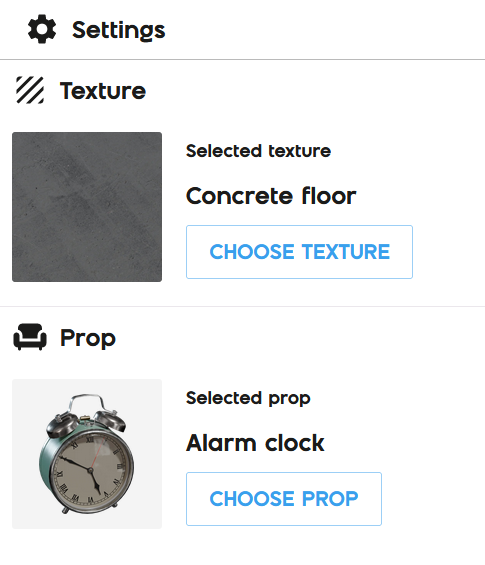
\includegraphics[width=.6\linewidth]{parts/developer-documentation/frontend/images/editorSettings.png}
    \label{fig:editorSettings}
  \end{minipage}%
  \begin{minipage}{.5\textwidth}
    \centering
    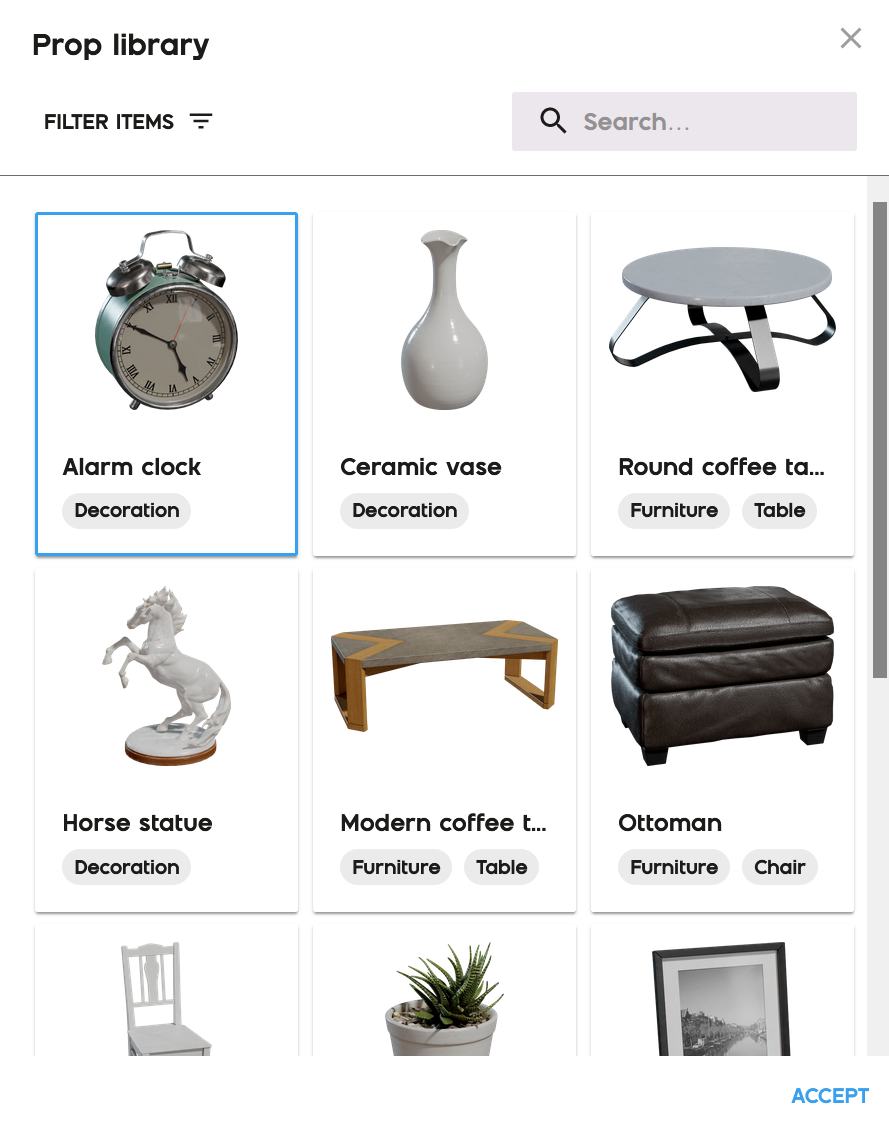
\includegraphics[width=.6\linewidth]{parts/developer-documentation/frontend/images/library.png}
    \label{fig:library}
  \end{minipage}
  \caption{Szerkesztő beállítások és a díszítőelem könyvtár ablak}
\end{figure}

\subsection{Fordítások}
Az Archytex alkalmazás több nyelven is elérhető. Az i18n\footnote{i18: Internationalisation, avagy nemzetközisítés}  megvalósításához az i18next nevű React könyvtárat használtuk. Az alkalmazás gyökérkomponensében importáltuk az nyelvekhez tartozó JSON fájlokat, amikben megtalálható az összes előforduló fordítási kulcs, amelyhez tartozik egy-egy hozzárendelt fordítás.

\begin{figure}[h]
  \centering
  \begin{minipage}{.7\textwidth}
    \centering
    \begin{lstlisting}
      i18n.use(initReactI18next).init({
        resources: {
          en: { translation: translationEn },
          hu: { translation: translationHu },
          jp: { translation: translationJp },
        },
        lng: "en",
        fallbackLng: "en",
        interpolation: { escapeValue: false },
      });\end{lstlisting}
  \end{minipage}
  \caption{Az i18next inicializálása angol, magyar és japán nyelvvel}
\end{figure}


\subsection{Tesztek}

% Editor
\section{Szerkesztő}
\rhead{Szerkesztő}

\subsection{Technológiák}

A 3D szerkesztő elkészítése számos technikai és tervezési problémát vetett fel. Egy olyan szoftver
megalkotása volt a cél, amely elég egyszerű ahhoz, hogy bárki használhassa, viszont megfelelően
eszköz dús ahhoz, hogy képes legyen bonyolult épületek tervezésére is. Ezen feltételek
megfogalmazása után arra jutottunk, hogy a 3D szerkesztőt egy web alapú alkalmazás keretein belül
fogjuk megvalósítani.

Egy ilyen szoftver esetében nagyon fontos a sebesség, ezért úgy döntöttünk, hogy a
böngészőkben használt JavaScript helyett a sokkal gyorsabb --- ámbár fiatalabb és éretlenebb ---
WebAssembly\footnote{\url{https://webassembly.org}} technológiát fogjuk használni. Mivel a
WebAssembly önmagában csak egy utasításkészlet, szükségünk volt egy programozási nyelvre,
amit lehetséges WebAssembly utasításokra fordítani. Erre a célra a
Rust\footnote{\url{https://www.rust-lang.org}}
programozási nyelvet választottuk. Ennek a döntésnek több oka is van:

\begin{itemize}
      \item Gyorsaság: A Rust egy rendszerközeli nyelv, hasonlóan a C-hez vagy C++-hoz, így rengeteg
            olyan optimalizáció valósítható meg, ami magasabb szintű nyelvekben nem lehetséges.

      \item Fejlett WebAssembly eszközök: Annak ellenére, hogy a nyelv viszonylag fiatal, rengeteg
            kiváló eszköz és könyvtár áll rendelkezésre a WebAssembly programok fejlesztésének
            elősegítéséhez. Ezek közül talán a legfontosabb a
            wasm-bindgen\footnote{\url{https://github.com/rustwasm/wasm-bindgen}} könyvtár, amellyel
            triviális feladattá válik a böngésző által használt JavaScript kód és a WebAssemblyre
            átforduló Rust kód összekötése.

      \item Tapasztalat: A fejlesztői csapat két tagja már használta a Rust programozási nyelvet a
            múltban, így elkerülhettük az új technológiák tanulásával járó problémákat.
\end{itemize}

\subsection{Működési elvek}

A használt technológiák kiválasztása után megkezdődött a szerkesztő működési elveinek felállítása.
Hamar eldöntöttük, hogy nagyrészt két, már létező szoftver eszközeiből szeretnénk ötleteket
meríteni.

Az egyik szoftver, a Blender egy általános rendeltetésű
háromdimenziós modellező program. Rendkívül sokoldalú és bonyolult, ezért csak néhány mechanizmust
ültettünk át a saját szerkesztőnkbe, például a kijelölés és a mozgatás módját.

\begin{figure}[H]
      \centering
      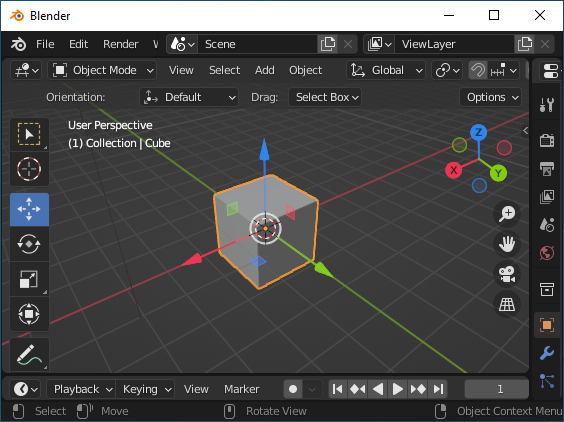
\includegraphics[width=0.5\textwidth]{parts/developer-documentation/editor/images/blender.png}
      \caption{Blender}
\end{figure}

A másik kiindulási pontként használt szoftver a Valve Hammer Editor. A
program a Valve Software által fejlesztett Source játékmotor pályaszerkesztő alkalmazása. A Hammer
Editor egyik erőssége, és egyben az a tulajdonsága, amit mi is megvalósítottunk az, hogy benne
bármilyen komplex beltéri vagy kültéri jelenet lemodellezhető kisebb, egyszerűbb alakzatok
felhasználásával.

\begin{figure}[H]
      \centering
      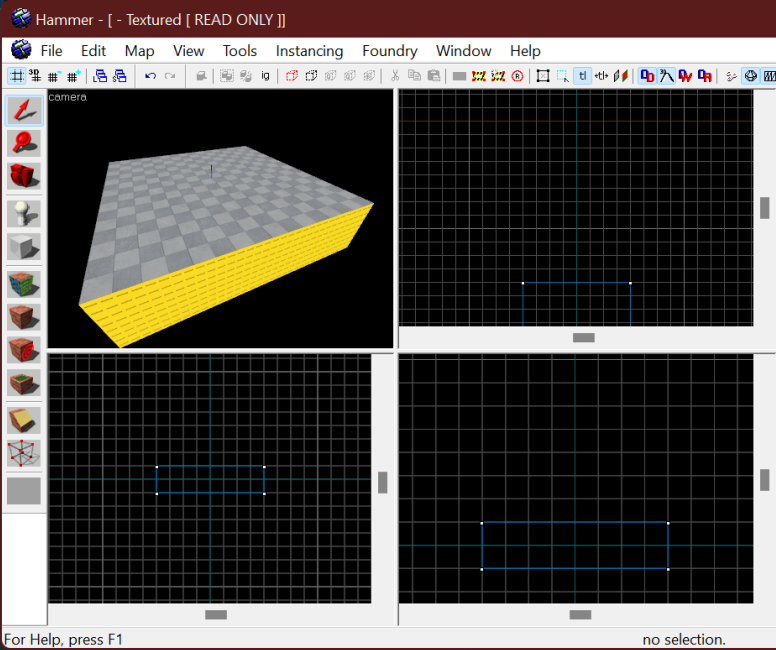
\includegraphics[width=0.5\textwidth]{parts/developer-documentation/editor/images/hammer.png}
      \caption{Valve Hammer Editor}
\end{figure}


\subsection{Kommunikáció a böngészővel}

Problémák és kihívások nem csak a tervezési fázisban bukkantak fel. Az egyik legelső probléma,
amivel fejlesztés közben találkoztunk, az a böngészővel való kommunikáció kérdése. Mivel a
JavaScript alapú felhasználói felület, és a Rust alapú szerkesztő valójában két független
alkalmazás, ezért ki kellett találni egy módszert az információmegosztásra. Az egyszerű
függvényhívások két okból nem feleltek meg. Először is, a JavaScript és WebAssembly kód natívan
csak egész számok átadására képes, ami mi céljainkhoz kevés. Másodszor, mivel a szerkesztő teljes
mértékben WebAssembly memóriában él, nincs semmilyen JavaScript objektum, aminek a függvényeit le
lehetne hívni.

Az első problémánkra a wasm-bindgen nevű Rust könyvtár adott megoldást. A wasm-bindgen lehetségessé
teszi az egész számoknál komplexebb adatstruktúrák átültetését Rust kódból JavaScript kódba, és
fordítva. A második probléma megoldása kicsit nehezebbnek bizonyult. Végül egy olyan
modellt valósítottunk meg, amiben a két fél két különböző módszert használ a kommunikációhoz.
Amikor a böngésző kommunikál a szerkesztővel, azt üzenetekkel teszi. Ezek az üzenetek egyszerű
adatstruktúrák amik egy aszinkron csatornán keresztül jutnak el a szerkesztőhöz. Amikor az
információátadás fordítva történik, a helyzet egyszerűbb: a JavaScript oldal egyszerűen átad egy
anonim függvényt a Rust oldalnak, amit aztán a szerkesztő szükség esetén meghív.

\subsection{3D grafika}

A szerkesztő egyik legfontosabb feladata, hogy képes legyen kirajzolni a jelenetet a képernyőre.
Ezt teszik lehetővé a különböző grafikus API-k, mint például az
OpenGL\footnote{\url{https://www.opengl.org}}, Vulkan\footnote{\url{https://www.vulkan.org}},
vagy böngésző esetén a WebGL\footnote{\url{https://www.khronos.org/webgl}}.
A Rust programozási nyelvhez rengeteg olyan könyvtár érhető el, ami ezeket az API-ikat elérhetővé
teszi. Mi úgy döntöttünk, hogy a wgpu\footnote{\url{https://github.com/gfx-rs/wgpu}} könyvtárat fogjuk
használni. Ennek legfőbb oka az, hogy egy letisztult, biztonságos réteget húz a régies WebGL
interfészre.

\pagebreak

\subsection{Művelet alapú szerkesztés}

Az előzetes tervezési fázisban számunkra fontos kikötés volt, hogy a szerkesztés közben
megvalósulhasson az ún. non-destruktív munkamenet. Ez azt jelenti, hogy bármit, amit a felhasználó
megtesz, azt vissza lehet vonni. Ahhoz, hogy ez lehetséges legyen, valamilyen formában el kell
tárolni a múltbeli szerkesztési lépéseket. Végül úgy döntöttünk, hogy az egész szerkesztőt ezen
alapelv köré építjük fel. Létrehoztunk egy speciális adatszerkezetet, amely az összes elvégezhető
szerkesztési lépést képes eltárolni. Amikor a felhasználó változtat valamit a jeleneten, egy
ilyen adatszerkezet (művelet) kerül átadásra. Az végrehajtás után a szerkesztő felépíti az művelet
ellentétét, az inverz műveletet. Végül az inverz művelet eltárolásra kerül egy ún. visszavonási
veremben. Amikor a felhasználó kiadja a visszavonási parancsot, a visszavonási verem tetején lévő
művelet (ha létezik) újra végrehajtásra kerül, és belekerül egy másodlagos verembe, ami a visszavont
műveletek inverzeit tárolja. Ez azért szükséges, mert visszavonás mellet ismétlés is lehetséges.

\begin{figure}[H]
      \centering
      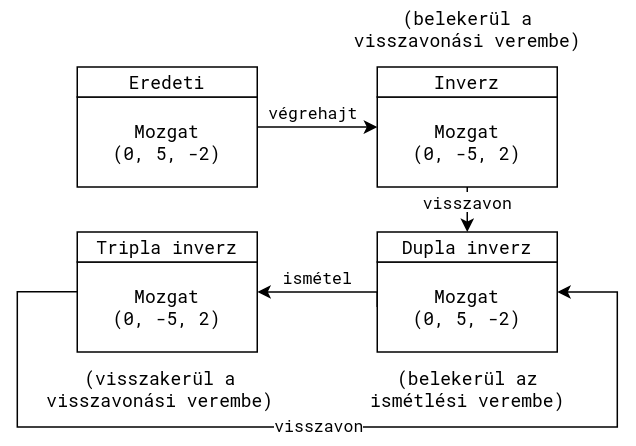
\includegraphics[width=0.5\textwidth]{parts/developer-documentation/editor/images/actions.png}
      \caption{A művelet alapú szerkesztés folyamatábrája}
\end{figure}

\subsection{Külső erőforrások kezelése}

A tervezési fázisban hamar kiderült, hogy sok időt és energiát kell fektetnünk a szerkesztő által
használt külső erőforrások tárolásának és létrehozásának módjának meghatározásába. Arra jutottunk,
hogy ezen célok teljesítéséhez saját fájlformátumokat fogunk kifejleszteni. A fejlesztés során
felmerülő igények kielégítésére végül három új fájlformátum született meg: .ascn, .amdl, és .agzm.
Mindhárom fájlformátum bináris kódolású, előállításukat és beolvasásukat a
bincode\footnote{\url{https://github.com/bincode-org/bincode}}
könyvtár végzi. Az adatokat mindegyik formátum egymásba ágyazott struktúrákban tárolja.

\pagebreak

\subsubsection{Jelenetfájl (.ascn)}

Az első általunk fejlesztett fájlformátum, a .ascn arra szolgál, hogy a szerkesztőben készített
3D jeleneteket tárolja. Az egész adatszerkezet egyetlen \emph{Scene} nevű struktúrában helyezkedik
el. Ennek a struktúrának két eleme van: \emph{camera} és \emph{world}. A \emph{Camera} struktúrában
a kamera pozíciója és forgása tárolódik, míg a \emph{World} struktúra kicsit bonyolultabb. Szintén
két eleme van: \emph{solids} és \emph{props}. Mindkét elem vektoros adatszerkezet, azaz
határozatlan mennyiségű homogén adatot tárol.

A \emph{solids} elem \emph{Solid} típusú struktúrákat tárol. Egy \emph{Solid} példány egy primitív
szilárd alakzatot modellez. Tartalmazza az alakzat csúcsait és lapjait, emellett a lapok textúráit.

A \emph{props} elem \emph{Prop} típusú struktúrákat tárol. Egy \emph{Prop} példány egy díszítőelem
adatait tárolja. Egy díszítőelemnek modell ID-je, pozíciója és forgása van.

\begin{figure}[H]
      \centering
      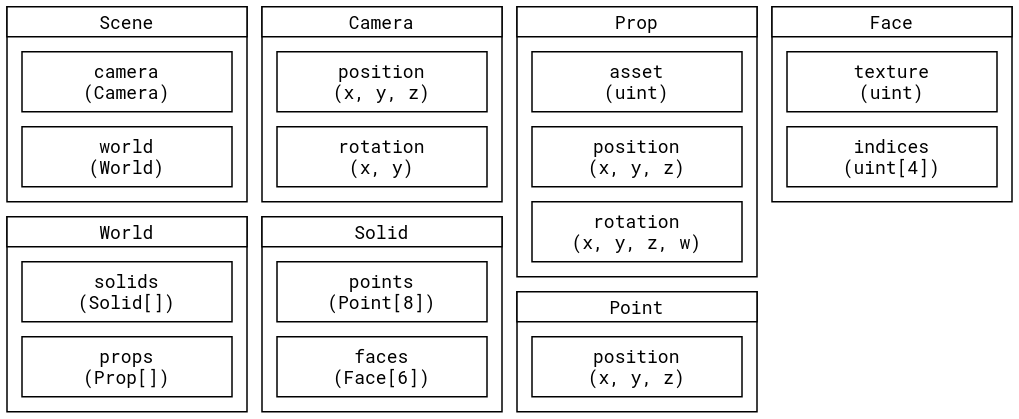
\includegraphics[width=0.8\textwidth]{parts/developer-documentation/editor/images/ascn.png}
      \caption{A .ascn fájlformátum adatszerkezetei}
\end{figure}

\pagebreak

\subsubsection{Modellfájl (.amdl)}

A .amdl fájlformátum egy tetszőlegesen komplex 3D modell tárolására szolgál, néhány korlátozással.
A formátum például nem képes animációkat kódolni, hiszen a szerkesztő nem támogatja a mozgó tárgyak
megjelenítését. A modellfájl gyökérstruktúrája \emph{Prop} névre hallgat. Két eleme van:
\emph{bounds} és \emph{meshes}. A \emph{bounds} elem a modell köré írható,
tengelyekhez igazított téglatestet tárolja. A \emph{meshes} elem vektoros adatszerkezet, ami a
modellt felépítő, textúrázott almodelleket tárolja.

\begin{figure}[H]
      \centering
      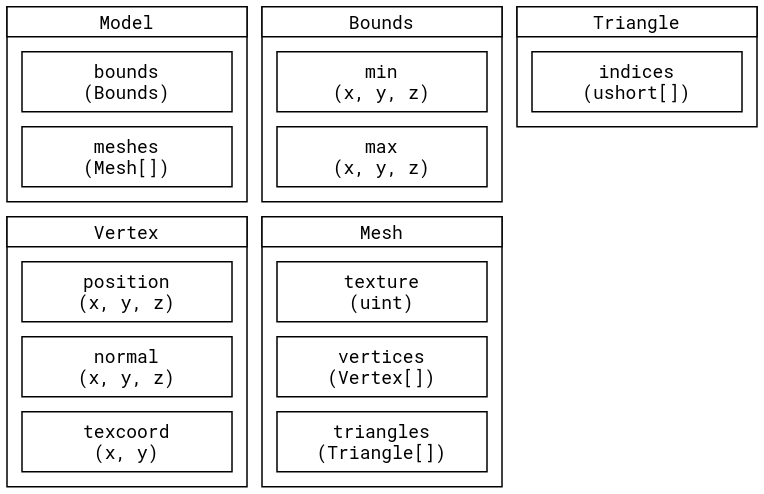
\includegraphics[width=0.6\textwidth]{parts/developer-documentation/editor/images/amdl.png}
      \caption{A .amdl fájlformátum adatszerkezetei}
\end{figure}

\subsubsection{Gizmofájl (.agzm)}

Az Archytex szerkesztő forráskódjában a gizmo szónak két jelentése is van: hivatkozhat az egér
általi mozgatást elősegítő alakzatokra, de arra a speciális 3D modellre is, aminek nincsenek
almodelljei és textúrái sem. A gizmofájl az utóbbi modellek tárolására szolgál. A három saját
fájlformátum közül ez a legegyszerűbb, hisz csak egyszerű geometriát kódol: csúcsokat, és az
azokból alkotott háromszögeket.

\begin{figure}[H]
      \centering
      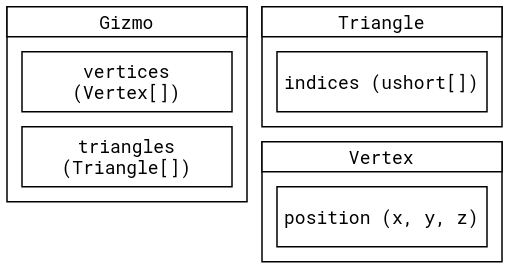
\includegraphics[width=0.4\textwidth]{parts/developer-documentation/editor/images/agzm.png}
      \caption{A .agzm fájlformátum adatszerkezetei}
\end{figure}

% Ray-tracer
\section{Online renderelő}
\rhead{Online renderelő}
\label{raytracer}

Az épületek bemutatásának elősegítésének érdekében szerettünk volna egy valósághű képalkotó programot létrehozni, amely beépül a honlapba és a szerkesztőbe is. Erre a célra egy hálózaton elosztott Path Tracer-t írtunk a Rust nevű programozásnyelvben.

\subsection{Raytracer}
Az elmúlt pár évben kifejezetten felkapott lett a \emph{Raytracing} kifejezés. Ezt a Nvidia RTX videókártyáinak megjelenése segítette elő, hiszen ez az első olyan eszköz, amely képes ezt a folyamatot valós-idejűleg megcsinálni. 

A raytracing egy módszer három dimenziós képek létrehozására. Egy másik gyakran használt módszer a raszterizálás, amit általában a játékok és más valósidejű szoftverek (így a mi szerkesztőnk) használnak, mert gyorsabb, de nem olyan sokoldalú, mint a raytracing.

\subsubsection{A módszer leírása}
A raytracing lényege, hogy a kamera képének minden egyes pixeléből egy-egy sugarat "lövünk" ki és megnézzük, hova landol. Landolás után a sugárhoz tartozó pixelt a landolás helye és az ott lévő felület szerint beszínezzük.

E szerint három fő komponense van egy ilyen rendszernek: egy kamera, egy módszer a sugarak landolási helyének eldöntéséhez és egy módszer a pixelek beszínezésére. A raytracerek sokoldalúságát az adja, hogy sokféle komponens létezik amely ezeket a feladatokat felveheti. Teljesen árnyékmentes, csak gömbökkel foglalkozó lyukkamerát használó megoldásoktól kezdve egészen a valósággal összehasonlíthatatlan képeket generáló megoldásokig mindenre képes a megfelelő komponensekkel.

\subsubsection{Gyorsító struktúrák}

A fent említett három komponens közül a a sugár landolásának megkeresése jár a legnagyobb költséggel, hiszen ezt pixelenként kell megnézni, akár többször is.

Az Archytex-ben háromszögekből álló modellekkel dolgozunk. Ha a gép meg szeretné tudni, hogy egy sugár hol találkozik a modell akármelyik részével, akkor mindegyik háromszöget egyenként meg kell nézni. Ez egy összetettebb épület esetén megtöbbszörözheti a feldolgozási időt. 

Ennek az időnek a lecsökkentésére különböző gyorsító struktúrákat használhatunk. Manapság a leggyakoribb ilyen struktúra a Bounding Volume Hierarchy (BVH).

A BVH lényege, hogy minden háromszöghöz hozzárendelünk egy téglatestet (1. szint), amelybe belefér, majd az egymás mellett lévő téglatesteket párokba helyezzük és azokat is téglatestekbe helyezzük (2. szint). Ezt addig folytatjuk, amíg végül csak egy téglatest marad hátra. 

A sugarak feldolgozásakor először leellenőrizzük, hogy eltalálja-e a külső téglatestet. Ha nem találja el, akkor a háromszögek közül sem találhatta el egyiket se. Ha a téglatestet eltalálta, akkor az abban lévő téglatestekkel is meg kell tennünk ugyan ezt az ellenőrzést. Ennek az előnye, hogy átlagosan az algoritmus komplexitása $O(n)$-ről $O(log(n))$-re csökkent.

\subsection{Rust}
A renderelő rendszer elkészítéséhez Rustot használtunk. Ennek több oka is van:

Mint a szerkesztőnél, itt is fontos szempont volt a gyorsaság, hiszen minél kevesebb önköltsége van a programozási nyelvnek, annál gyorsabbra lehet írni az algoritmusokat.

Ezzel szemben lényeges a biztonság is. A C és a C++ gyors, rendszerközeli nyelvek, de nem érkeznek ugyanazokkal a biztonsági garanciákkal, mint a Rust. Ez nem előnyös egy online renderer esetén, hiszen a felhasználótól kéri az adatokat és olyan környezetben fut ahol el lehet érni bizalmas adatokat. C és C++ esetén bizonyos programhibákkal egy támadó képes lehet átvenni az irányítást a szerver felett és más felhasználók adatait ellopni.

Fontos még kiemelni a Rust generikus rendszerét, amely elősegíti a fent említett komponensek különvételét és egybeágyazását különféle compile idejű optimalizációkkal.

\subsection{Pathtracer}
A raytracerek segítségével lehet a fény viselkedését is szimulálni. Ezt hívjuk Path Trace-nek.

Lényege, hogy a kamerából kijövő sugaraknak hagyjuk, hogy a felületre érkezve folytassák utukat egy másik irányba. Ez az irány a felület tulajdonságaitól függ. Egy tükör a sugarat csak egy irányba küldheti tovább, míg egy téglafal a fényt szórja, tehát több lehetséges iránya is van a fénynek. 

A helyes megjelenítéshez a lehetséges irányok terén kell integrálni az egyes irányokhoz tartozó értékeket, az adott irány szerint súlyozva. Ez egy olyan integrálási probléma, amelynek nincs tényleges megoldása, csak megközelíteni tudjuk.

Erre a megközelítésre létezik a Monte Carlo integrálás. Lényege, hogy a lehetséges irányok közül egy megadott darabot (sample szám) kiválasztunk véletlenszerűen, majd azokat átlagoljuk.

Az így keletkezett kép a várt képnek csak egy megközelítése. Minősége a sample számtól függ. Alacsony sample szám esetén a kép zajos lehet, magas sample szám esetén a feldolgozás ideje megnőhet.

\subsubsection{Open Image Denoise}
Hogy alacsony sample szám esetén is viszonylag jó minőségű képeket kapjunk, az Intel által fejlesztett Open Image Denoise\footnote{\url{https://www.openimagedenoise.org/}} nevű szoftvert használjuk. 

Ez a szoftver mesterséges intelligenciát használ a képen lévő zaj eltávolítására.

Csak x86 alapú rendszereken elérhető.

\todo[inline]{Példa}

\subsection{Elosztott renderelő}

A képek elkészítési idejének csökkentésére a renderelőhöz hozzáadtunk egy elosztási rendszert.

Ez a rendszer RabbitMQ-ra\footnote{\url{https://www.rabbitmq.com/}} és Redis-re\footnote{\url{https://redis.io/}} épül. A RabbitMQ egy üzenetküldő rendszer, amely a különböző rétegek közti kommunikációt segíti elő, míg a Redis egy kulcs-érték adatbázis, a hosszabb ideig szükséges és nagyobb adatok tárolására.

A Redis szerverhez hozzáadtuk a RedisAI\footnote{\url{https://oss.redis.com/redisai/}} kiegészítőt, amivel lehet tömbökön végrehajtani matematikai operációkat. Ez a későbbiekben még hasznos lesz.

Az egyszerűbb kezelés érdekében, két különböző réteget hoztunk létre: a tartomány kezelő réteg (domain manager) és a feliratkozó réteg (subscriber)

\subsubsection{Tartománykezelő réteg}
A Tartománykezelő réteg feladata a renderelési kérések fogadása a backendtől, munkákra osztása és a összerakása.

A renderelés elkezdéséhez egy véletlenszerű azonosítót kell generálnunk a kérésünk számára (ID) és Redis-ben a következő értékeket kell beállítanunk:

\begin{itemize}
    \item archyrt:ID:width
    
    A várt kép szélessége pixelben
    \item archyrt:ID:height
    
    A várt kép magassága pixelben
    \item archyrt:ID:samples
    
    A renderelés során használt sample-ök száma
    \item archyrt:ID:scene
    
    A projekt által haszált .ASCN bináris fájl
\end{itemize}

A kéréseket a RabbitMQ \emph{archyrt:dispatch} sorából várja. Az innen beérkező üzenetek karakterláncok, amelynek formátuma:\emph{kérésID\#felhasználóID\#projektID}.

Ekkor a tartománykezelő a képet felosztja 16 egyenlő részre (csempe), és minden rész minden egyes samplejéhez egy-egy munkát köt a saját egyedi azonosítójával. A munkákat a \emph{archyrt:taskqueue} sorba küldi, a következő formátummal:\linebreak\emph{kérésID\#munkaID\#visszatérésiSorNeve\#csempeXKoordinátája\#csempeYKoordinátája}.

A fenti üzenetben megadott sorból egyenként elfogadja az üzeneteket, az üzenetből kiolvassa, hogy a munka során generált kép hova lett mentve, és feldolgozza azt.\linebreak \emph{RedisKulcsAholAKépVan\#CsempeX\#CsempeY}

Ezek után a tartománykezelő végrehajtja a zajeltávolítást és elmenti a képet a fájlrendszerre.

\subsubsection{Feliratkozó réteg}
A feliratkozó réteg feladata a Tartománykezelő által kiadott munkák végrehajtása. 

Miután megkapta a feladatot az \emph{archyrt:taskqueue} sorból (lásd fent), betölti a Redis-ből a kéréshez tartozó jelenetet és kirendereli. Renderelés után feltölti Redis adatbázisba tensorként, véletlenszerű kulccsal és ezt jelzi a tartománykezelőnek.

\appendix
\part{Irodalomjegyzék}
\rhead{Irodalomjegyzék}

\lipsum*[1-6]


\rhead{}
\bibliographystyle{plain}
\bibliography{ref}
\end{document}